\section{Vysvětlete, co je přirozená vinětace. Projevuje se přirozená vinětace více u normálních objektivů nebo u 
širokoúhlých objektivů?}.

\begin{figure}[H]
  \center
  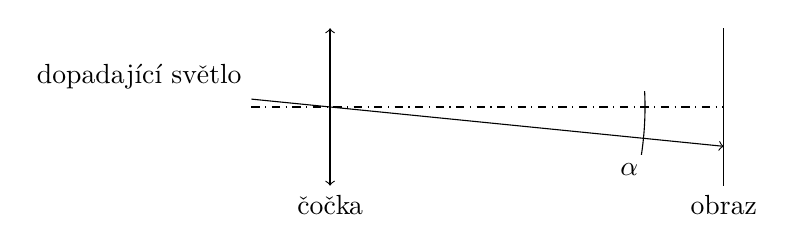
\begin{tikzpicture}
    \draw[dashdotted] (-1,0) -- (5,0);
    \draw[<->] (0,-1) node[below] {čočka} -- (0,1);
    \draw (5,-1) node[below] {obraz} -- (5,1);
    \draw[->] (-1,0.1) node[above left] {dopadající světlo} -- (5,-0.5);
    \begin{scope}
      \clip (3.5,-0.6) rectangle (4.5,0.2);
      \draw (0,0) circle (4);
    \end{scope}
    \node at (3.8,-0.8) {$\alpha$};
  \end{tikzpicture}
\end{figure}
\begin{itemize}
  \item
    Přirozenou vinětaci popisuje činitel $\cos(\alpha)^4$.
  \item
    Paprsky s větším úhlem $\alpha$ jsou více blokovány.
  \item
    Projevuje se více u širokoúhlých oběktivů.
  \item
    Lze ji kompenzovat kalibrací kamery.    
\end{itemize}
